%-----------------------------------------------------------------------
%
%   UFRJ  - Universidade Federal do Rio de Janeiro
%   COPPE - Coordena��o dos Programas de P�s-gradua��o em Engenharia
%   PEE   - Programa de Engenharia El�trica
%
%   COE-835  Controle adaptativo
%
%   Relat�rio da simula��o
%                                                         Ramon R. Costa
%                                                         05/out/09, Rio
%-----------------------------------------------------------------------
\documentclass[11pt,a4paper]{article}
\usepackage[latin1]{inputenc} %pacote para utilizar palavras acentuadas
\usepackage{amsmath,amssymb}  %pacotes do AMS
\usepackage{latexsym}         %pacote para incluir s�mbolos (ex.\Box)
\usepackage{fancybox,fancyhdr}%pacote com frescuras
\usepackage{graphicx}         %pacote para incluir figuras tipo eps
\usepackage[portuguese]{babel}
\usepackage{xcolor}
\usepackage{float}
\usepackage[a4paper]{hyperref}% Make sure it comes last of your loaded packages
\hypersetup{
  verbose,
  plainpages=false,
  bookmarks=true,
  colorlinks=true,
  linkcolor=blue
}

\input{macros}

\begin{document}
%---------------------------------------------------------------------
\pagestyle{fancy}%
\renewcommand{\headrulewidth}  {0.4pt}%
\renewcommand{\footrulewidth}  {0.4pt}%
\lhead{\bfseries{Relat�rio das simula��es}}%
\chead{}%
\rhead{\bfseries\thepage}%
\lfoot{}%
\cfoot{}%
\rfoot{[\hours] \quad \today}%
%---------------------------------------------------------------------
\begin{center}
  \huge{COE-835  Controle  adaptativo}  \\[20mm]

  \Large{Simula��es do Trabalho 1} \\[20mm]
\end{center}


Algoritmo: \quad \HI{Gradiente normalizado}

\bigskip%
Caso: \quad \parbox[t]{10cm}{
  $~n = 1$ \quad (ordem da planta) \\[2mm]
  $n^* = 1$ \quad (grau relativo) \\[2mm]
  $n_p = 1$ \quad (\# de par�metros) \\[20mm]
}

%---------------------------------------------------------------------

\tableofcontents

\newpage
%---------------------------------------------------------------------
%---------------------------------------------------------------------
\section{Resumo das equações do método}

%Abaixo, resumimos algumas das principais equações utilizadas no método.

\vspace{20mm}

\noindent

\equacao{Planta}
  {\dot{y}_p = a_p y_p + u \,, \quad P(s) = \frac{1}{s+a_p} \label{eq:planta}}

\equacao{Modelo}
  {\dot{y}_m = -a_m y_m + r \,, \quad M(s) = \frac{1}{s+a_m} \label{eq:ref_model}}

\equacao{Erro de saída}
  {e_0 = y_p - y_m \label{eq:error}}

\equacao{Lei de controle}
  {u = \theta \, y_p + r \label{eq:ctrl_law}}

\equacao{Filtro}
  {\dot{\zeta} + a_f \, \zeta = y_p \,, \quad F(s) = \frac{1}{s+a_f} \label{eq:filter}}

\equacao{Estimativa do erro}
  {\hat{e} = F(s) \odot \{\theta \, y_p\} - \theta\zeta \label{eq:est_error}}

\equacao{Erro de estimativa}
  {\varepsilon = e_0 - \hat{e} \label{eq:error_est}}

\equacao{Sinal normalizante}
  {m^2 &= 1 + \zeta^2 \\ m^2 &= 1 + \zeta^2 + \dot{\zeta}^2 \label{eq:norm_signal}}

\equacao{Lei de adaptação}
  {\dot{\theta} = - \frac{\gamma \varepsilon \zeta}{m^2} \label{eq:adpt_law}}

 \newpage
%---------------------------------------------------------------------
\section{Prova da limita��o de $\dot{\varepsilon}/m$}

Utilizando as eq.s do sistema, a din�mica do erro � expressa por:
%
\begin{flalign}
\dot{e}_0 &= \dot{y}_p - \dot{y}_m \nonumber \\
&= -a_m \, e_0 + \tilde{\theta} \, y_p \,,
\end{flalign}
%
ou ainda:
%
\begin{flalign}
e_0 &= \mathcal{L}^{-1}\left\{\frac{1}{s+a_m}\right\} \circledast ( \tilde{\theta}\,y_p ) \nonumber \\ 
&= \mathcal{L}^{-1}\left\{\frac{1}{s+a_m}\right\} \circledast (\theta\,y_p) - \theta^* \, \zeta \,,
\end{flalign}
%
onde o operador $\mathcal{L}^{-1}\{*\}$ denota a transformada de Laplace inversa, $\circledast$ denota a opera��o de \textit{convolu��o} de sinais e $\theta^*$ � o ganho de realimenta��o ideal.
%
Assim, o erro de estimativa pode ser escrito como:
%
\begin{flalign}
\varepsilon &= e_0 - \hat{e} \nonumber \\ 
&=\mathcal{L}^{-1}\left\{\frac{1}{s+a_m}\right\} \circledast (\theta \, y_p) - \theta^* \, \zeta - \mathcal{L}^{-1}\left\{\frac{1}{s+a_m}\right\} \circledast (\theta \, y_p) + \theta \, \zeta \nonumber \nonumber \\
&= \tilde{\theta} \, \zeta \,.
\label{eq:erro_est}
\end{flalign}

A seguinte candidata � fun��o de Lyapunov � proposta:
%
\begin{equation}
2V(\tilde{\theta}) = \gamma^{-1} \, \tilde{\theta}^2 \ge 0
\end{equation}

Derivando e utilizando a lei de adapta��o proposta, tem-se:
%
\begin{flalign}
\dot{V} &= \gamma^{-1} \, \tilde{\theta} \, \dot{\theta} \nonumber \\
&= - \frac{\varepsilon^2}{m^2} \leq 0 \,,
\end{flalign}
%
onde \eqref{eq:erro_est} foi utilizado. Como $\dot{V}$ � apenas negativa \textit{semi-definida}, mostra-se que $\tilde{\theta} \in \mathcal{L}_{\infty}$.

\begin{lemma}
Sejam $a,b \in \mathbb{R}$ e $m^2 = 1+a^2+b^2$. Ent�o:
%
\begin{flalign}
\norm{\frac{a}{m}} \leq 1 \,, \quad \forall a,b \in \mathbb{R} \,, \nonumber \\
\norm{\frac{b}{m}} \leq 1 \,, \quad \forall a,b \in \mathbb{R} \,. \nonumber
\end{flalign}
%
\end{lemma}

Dividindo \eqref{eq:erro_est} por $m = \sqrt{1+\zeta^2+\dot{\zeta}^2}$, obtemos:
%
\begin{flalign}
\frac{\varepsilon}{m} = \tilde{\theta} \, \frac{\zeta}{m} \,.
\label{eq:erro_est2}
\end{flalign}

De acordo com o Lema 1 (para $a = \zeta$, $b=\dot{\zeta}$), $\norm{\zeta/m} \leq 1$ e, como $\tilde{\theta} \in \mathcal{L}_{\infty}$, ent�o 
$\varepsilon/m \in \mathcal{L}_{\infty}$.
%
A lei de controle pode ser expressa por:
\begin{equation}
\dot{\theta} = \dot{\tilde{\theta}} = \gamma \, \underbrace{\frac{\varepsilon}{m}}_{\in \mathcal{L}_{\infty}} \, \frac{\zeta}{m} \,.
\end{equation}
%
Como $\varepsilon/m \in \mathcal{L}_{\infty}$ e pelo Lema 1 $\norm{\zeta/m} \leq 1$, ent�o $\dot{\tilde{\theta}} \in \mathcal{L}_{\infty}$.
%
Finalmente, derivando \eqref{eq:erro_est} no tempo e divindo por $m$, obtemos:
%
\begin{flalign}
\frac{\dot{\varepsilon}}{m} = \underbrace{\dot{\tilde{\theta}}}_{\in \mathcal{L}_{\infty}} \, \frac{\zeta}{m} + \underbrace{\tilde{\theta}}_{\in \mathcal{L}_{\infty}} \, \frac{\dot{\zeta}}{m} \,.
\label{eq:erro_est3}
\end{flalign}

Novamente utilizando o Lema 1, mostra-se que os sinais constituintes de $\dot{\varepsilon}/m$ s�o limitados, e portanto $\dot{\varepsilon}/m \in \mathcal{L}_{\infty}$.
 \newpage
%---------------------------------------------------------------------
\section{Diagramas de blocos}


\begin{figure}[H]
  \centering
  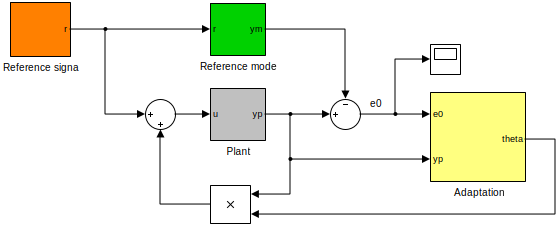
\includegraphics[width=14cm]{figs/blocks/MRAC_111_8_5.eps}
  \caption{Diagrama de blocos do sistema. \quad
  (Model: \HI{\texttt{MRAC-111.mdl}}) }
\end{figure}

%---------------------------------------------------------------------
\bigskip%
\begin{figure}[H]
  \centering
  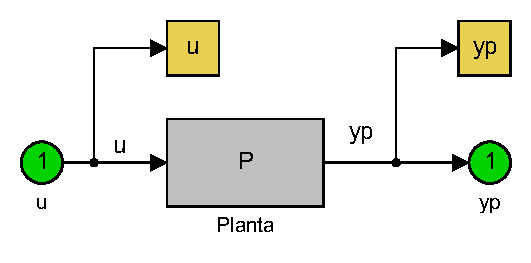
\includegraphics[scale=0.8]{figs/blocks/plant.eps}
  \caption{Diagrama de blocos da planta.}
\end{figure}

%---------------------------------------------------------------------
\bigskip%
\begin{figure}[H]
  \centering
  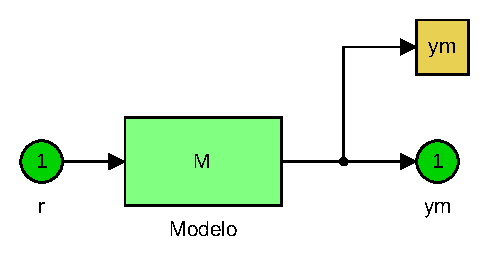
\includegraphics[scale=0.8]{figs/blocks/reference-model.eps}
  \caption{Diagrama de blocos do modelo de referência.}
\end{figure}

%---------------------------------------------------------------------
\bigskip%
\begin{figure}[H]
  \centering
  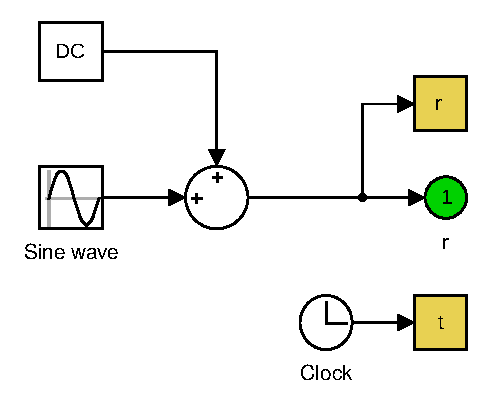
\includegraphics[scale=0.8]{figs/blocks/reference-signal.eps}
  \caption{Diagrama de blocos do gerador de sinais de referência.}
\end{figure}

%---------------------------------------------------------------------
\bigskip%
\begin{figure}[H]
  \centering
  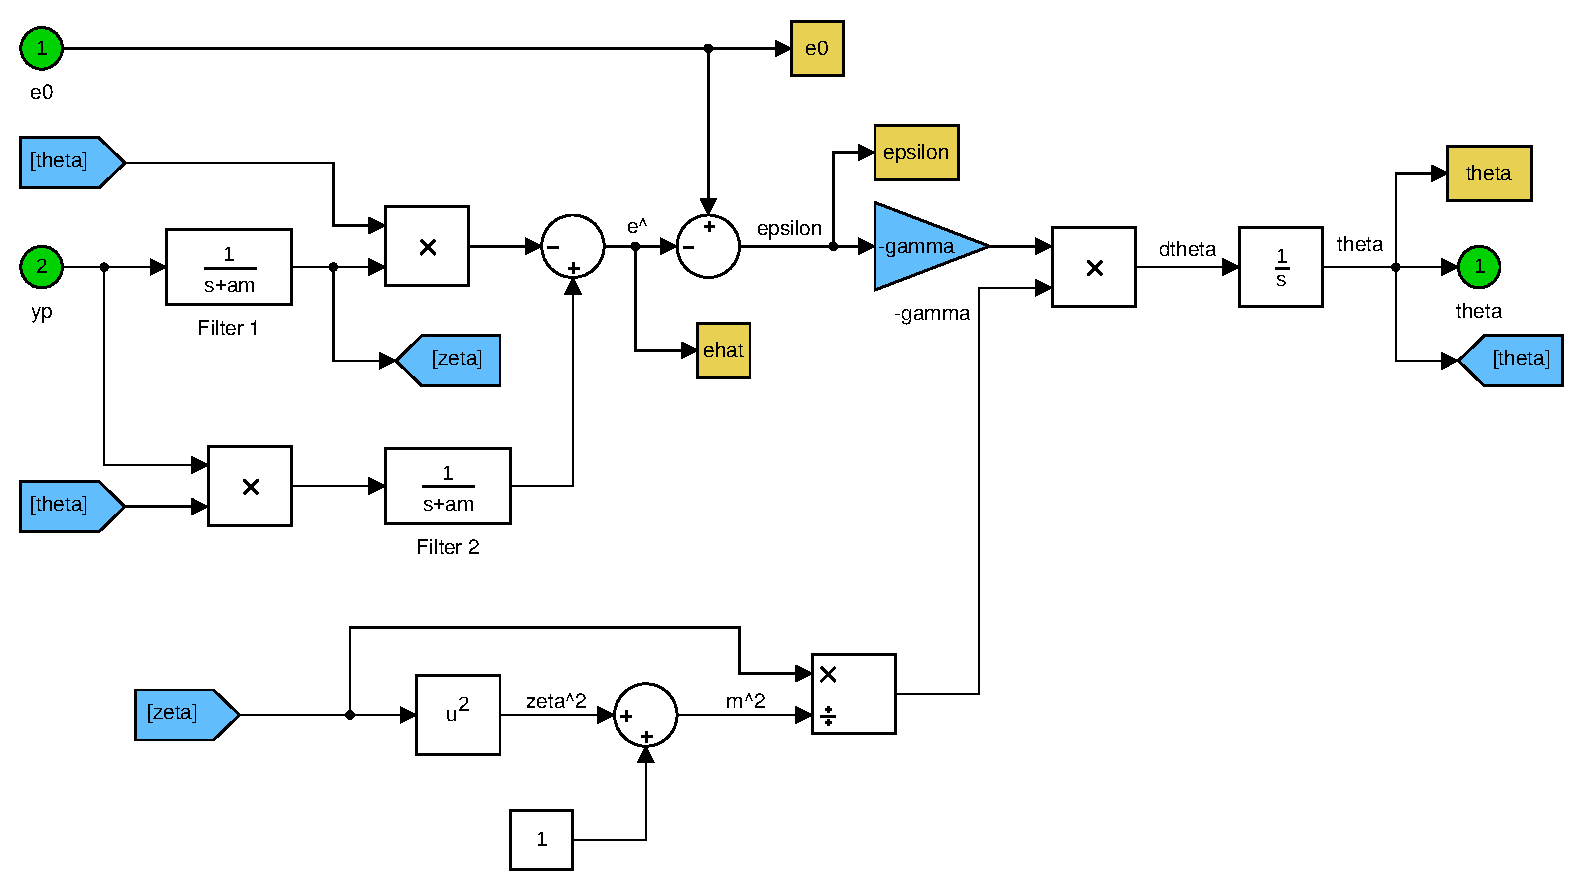
\includegraphics[width=16cm]{figs/blocks/adaptation.eps}
  \caption{Diagrama de blocos da lei de adaptação.}
\end{figure} \newpage
%---------------------------------------------------------------------
\section{Resultados das simula��es}

Simula��o utilizando \HI{\texttt{Matlab/Simulink}}.

\subsection{Simula��o \#1}

\bigskip%
Par�metros e condi��es iniciais  :
%
\begin{align*}
  a_p &= -2\,,  &  y_p(0) &= 0\,, & \theta(0) &= 0\,, \\
  a_m &= 1\,,   &  y_m(0) &= 0\,, & \gamma &= 10,\ 100\,, \\
  r &= 1\,.
\end{align*}

\bigskip%
\begin{figure}[H]
  \centering
  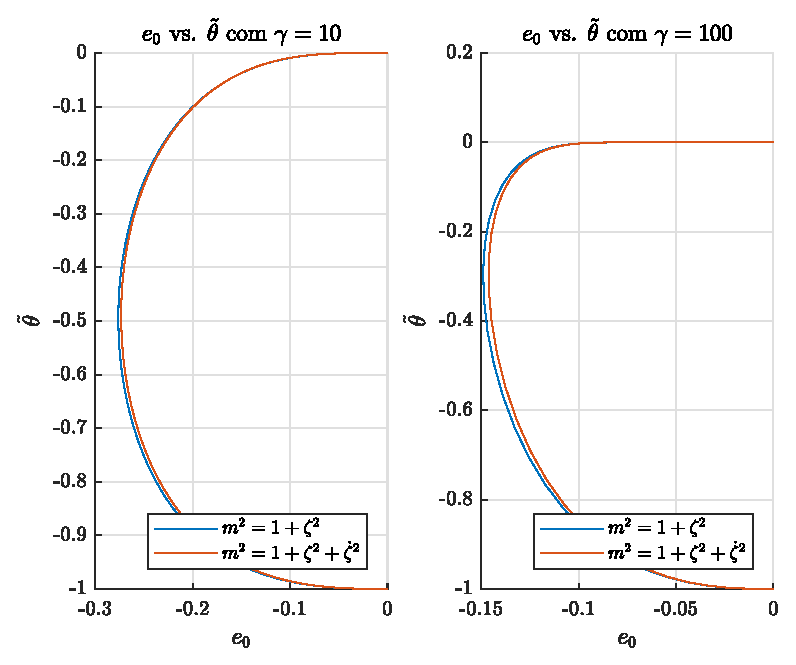
\includegraphics[width=12cm]{figs/fig01d.eps} \\[2mm]
  \caption{Diagrama $e_0 \times \tilde{\theta}$.
  \hfill (Script: \HI{\tt simu01.m}) }
\end{figure}

\newpage%
%---------------------------------------------------------------------
\begin{figure}[H]
  \centering
  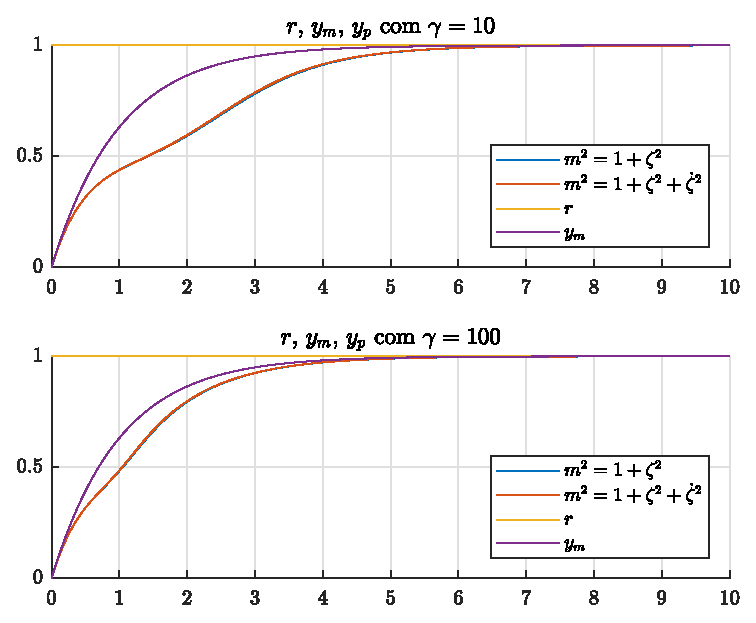
\includegraphics[width=12cm]{figs/fig01c.eps} \\[2mm]
  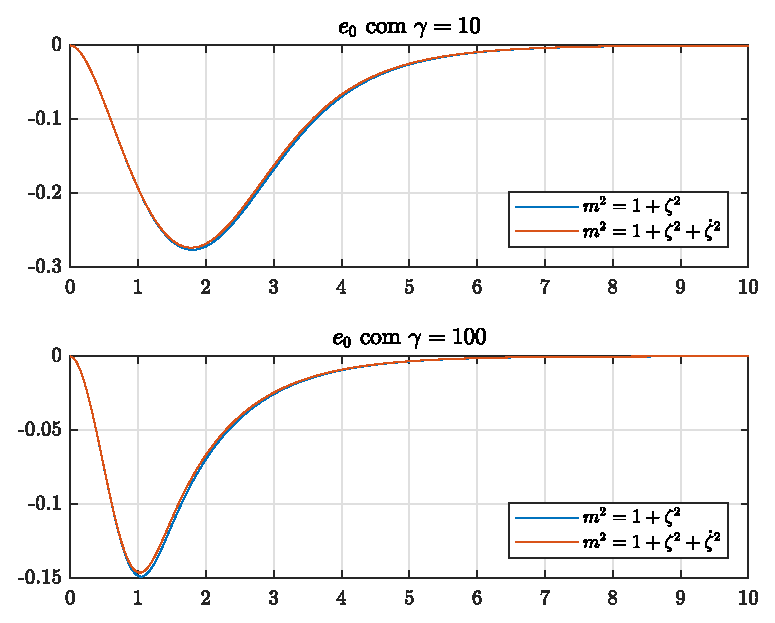
\includegraphics[width=12cm]{figs/fig01a.eps} \\[2mm]
  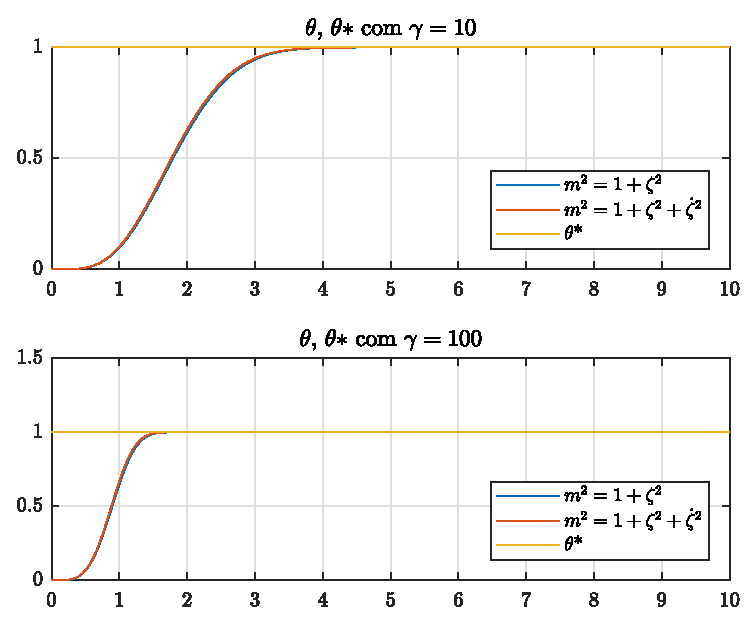
\includegraphics[width=12cm]{figs/fig01b.eps} \\[2mm]
  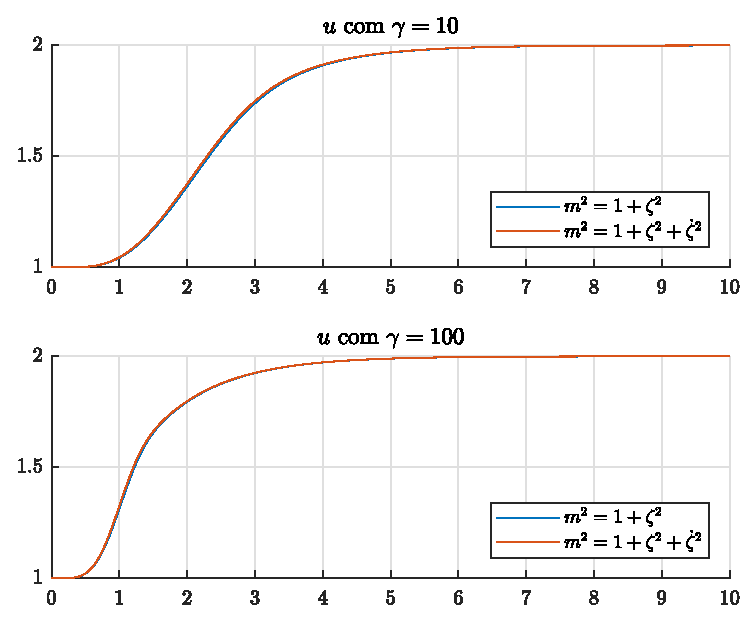
\includegraphics[width=12cm]{figs/fig01e.eps} \\[2mm]
  \caption{Resultado da simula��o com algoritmo Gradiente normalizado.
  \hfill (Script: \HI{\tt simu01.m}) }
\end{figure}


\newpage%
%---------------------------------------------------------------------
\subsection{Simula��o \#2}

\bigskip%
Par�metros e condi��es iniciais  :
%
\begin{align*}
  a_p &= -2\,,  &  y_p(0) &= \HI{2}\,, & \theta(0) &= 0\,, \\
  a_m &= 1\,,   &  y_m(0) &= 0\,, & \gamma &= 2,\ 100\,, \\
  r &= 1\,.
\end{align*}

\bigskip%
\begin{figure}[H]
  \centering
  \includegraphics[width=12cm]{figs/fig02d.eps} \\[2mm]
  \caption{Diagrama $e_0 \times \tilde{\theta}$.
  \hfill (Script: \HI{\tt simu02.m}) }
\end{figure}

\newpage%
%---------------------------------------------------------------------
\begin{figure}[H]
  \centering
  \includegraphics[width=12cm]{figs/fig02c.eps} \\[2mm]
  \includegraphics[width=12cm]{figs/fig02a.eps} \\[2mm]
  \includegraphics[width=12cm]{figs/fig02b.eps} \\[2mm]
  \includegraphics[width=12cm]{figs/fig02e.eps} \\[2mm]
  \caption{Resultado da simula��o com algoritmo Gradiente normalizado.
  \hfill (Script: \HI{\tt simu02.m}) }
\end{figure}

\newpage%
%---------------------------------------------------------------------
\subsection{Simula��o \#3}

\bigskip%
Par�metros e condi��es iniciais  :
%
\begin{align*}
  a_p &= -2\,,  &  y_p(0) &= \HI{10}\,, & \theta(0) &= 0\,, \\
  a_m &= 1\,,   &  y_m(0) &= 0\,, & \gamma &= 2,\ 100\,, \\
  r &= 1\,.
\end{align*}

\bigskip%
\begin{figure}[H]
  \centering
  \includegraphics[width=12cm]{figs/fig03d.eps} \\[2mm]
  \caption{Diagrama $e_0 \times \tilde{\theta}$.
  \hfill (Script: \HI{\tt simu03.m}) }
\end{figure}

\newpage%
%---------------------------------------------------------------------
\begin{figure}[H]
  \centering
  \includegraphics[width=12cm]{figs/fig03c.eps} \\[2mm]
  \includegraphics[width=12cm]{figs/fig03a.eps} \\[2mm]
  \includegraphics[width=12cm]{figs/fig03b.eps} \\[2mm]
  \includegraphics[width=12cm]{figs/fig03e.eps} \\[2mm]
  \caption{Resultado da simula��o com algoritmo Gradiente normalizado.
  \hfill (Script: \HI{\tt simu03.m}) }
\end{figure}
%---------------------------------------------------------------------
%\bibliographystyle{agsm}
%\bibliography{bib,coe736}

%---------------------------------------------------------------------
\end{document}
